% P1 学术写作版（2026-11-24）：实验结果与讨论。
% 由 chapter_04_results_rev_p0_20261124.tex 改写：按四个科学问题组织，结果段“发现→证据→异质性→解释”；
% 全部负结果与方法学限制保留，局限集中于4.7.4。数值来源：REV_P0 T1–T8、P1 T9–T11 与原始CSV，
% 逐句映射见 P1_20261124/P1_EVIDENCE_MAP_20261124.md。图4.1/4.2为pgfplots，数据直接取自T1/T3。未编译。
\section{实验结果与讨论}
\label{sec:cc-results-p1}

本节按引言的四个问题组织。除特别说明外，DLPFC结果的汇总方式是：每张切片先平均其随机种子，再对12张切片等权平均，同时给出3名供体各自的均值；乳腺癌结果先在患者内平均3个种子，再对6名患者等权平均。凡属事后分析（第\ref{subsec:cc-posthoc-p1}节）的结果均在文中注明。

\subsection{邻域表征：收益集中于最近邻层，深层增益有限且因切片而异}
\label{subsec:cc-res-neighborhood-p1}

\paragraph{累计深度。}在参考类别数条件下，邻域信息的收益主要来自第一层邻域（表\ref{tab:cc-depth-p1}，图\ref{fig:cc-depth-donor-p1}）。从仅用自身表示的5维$L_0$增加第一层邻域后，ARI由0.3051升至0.4081，NMI由0.4133升至0.5422；这一提升在12张切片和3名供体中方向一致，是整个深度范围内最大的一步。继续加深到15、20、25维时，宏平均ARI依次为0.4299、0.4383、0.4418，增量缩小到0.004--0.022。这些增量小于切片间标准差（0.060--0.072），与切片内种子标准差（0.023--0.037）处于同一量级。在切片层面，15维之后的方向并不一致：12张切片中有6张25维的ARI低于15维；供体D3的ARI则随深度增加而下降（15、20、25维依次为0.465、0.459、0.448）。

\begin{table}[htbp]
\centering
\caption{参考类别数条件下累计邻域深度的聚类表现。SD为切片间标准差；种子SD为切片内GMM种子标准差的平均值；D1--D3为各供体4张切片的ARI均值}
\label{tab:cc-depth-p1}
\small
\begin{tabular}{lcccccccc}
\toprule
邻域特征 & 维度 & ARI & SD & 种子SD & NMI & D1 & D2 & D3\\
\midrule
$L_0$ & 5 & 0.3051 & 0.063 & 0.023 & 0.4133 & 0.338 & 0.238 & 0.339\\
$L_0$--$L_1$ & 10 & 0.4081 & 0.066 & 0.037 & 0.5422 & 0.409 & 0.368 & 0.448\\
$L_0$--$L_2$（A） & 15 & 0.4299 & 0.072 & 0.032 & 0.5780 & 0.429 & 0.396 & 0.465\\
$L_0$--$L_3$ & 20 & 0.4383 & 0.060 & 0.027 & 0.5891 & 0.455 & 0.401 & 0.459\\
$L_0$--$L_4$ & 25 & 0.4418 & 0.066 & 0.028 & 0.5982 & 0.475 & 0.402 & 0.448\\
\bottomrule
\end{tabular}
\end{table}

\begin{figure}[htbp]
\centering
\begin{tikzpicture}
\begin{axis}[width=0.78\linewidth,height=6.2cm,xlabel={邻域特征维度（层数$=$维度$/5-1$）},ylabel={ARI},
  xtick={5,10,15,20,25},ymin=0.2,ymax=0.5,legend pos=south east,legend cell align=left,grid=major,grid style={gray!25}]
\addplot[thick,black,mark=*] coordinates {(5,0.3051)(10,0.4081)(15,0.4299)(20,0.4383)(25,0.4418)};
\addlegendentry{12切片宏平均}
\addplot[blue,mark=square*] coordinates {(5,0.3382)(10,0.4090)(15,0.4291)(20,0.4551)(25,0.4750)};
\addlegendentry{供体D1}
\addplot[red,mark=triangle*] coordinates {(5,0.2381)(10,0.3677)(15,0.3958)(20,0.4012)(25,0.4024)};
\addlegendentry{供体D2}
\addplot[teal,mark=diamond*] coordinates {(5,0.3390)(10,0.4476)(15,0.4648)(20,0.4587)(25,0.4480)};
\addlegendentry{供体D3}
\end{axis}
\end{tikzpicture}
\caption{参考类别数条件下ARI随累计邻域深度的变化（每切片先平均10个GMM种子；数据来源：REV\_P0汇总表T1）。第一层邻域带来最大且一致的提升，15维之后供体间方向不一致}
\label{fig:cc-depth-donor-p1}
\end{figure}

\paragraph{等维组成。}在维度固定为15维时，邻域块组成的差别小于切片之间的差别（表\ref{tab:cc-equaldim-p1}）。6种15维组合的宏平均ARI在0.424--0.437之间，NMI在0.578--0.590之间，极差约0.013，远小于切片间标准差；含远邻块的组合（如$[L_0,L_1,L_3]$，ARI 0.4374）与20维累计配置（0.4383）接近。逐切片看，ARI最高的15维组合分布在全部6种之间（A与$[L_0,L_2,L_4]$各3张，B与$[L_0,L_2,L_3]$各2张，其余两种各1张），没有一种组合稳定占优。

\begin{table}[htbp]
\centering
\caption{参考类别数条件下6种15维邻域组合的表现（12切片等权均值）}
\label{tab:cc-equaldim-p1}
\small
\begin{tabular}{lcccccc}
\toprule
 & A $[L_0,L_1,L_2]$ & $[L_0,L_1,L_3]$ & B $[L_0,L_1,L_4]$ & $[L_0,L_2,L_3]$ & $[L_0,L_2,L_4]$ & $[L_0,L_3,L_4]$\\
\midrule
ARI & 0.4299 & 0.4374 & 0.4332 & 0.4244 & 0.4280 & 0.4251\\
NMI & 0.5780 & 0.5862 & 0.5889 & 0.5821 & 0.5897 & 0.5833\\
\bottomrule
\end{tabular}
\end{table}

\paragraph{开发阶段候选组合的检验。}组合B（以远邻块$L_4$替换$L_2$）是在开发切片151507上看到ARI高出0.047之后提出的候选。扩展到全部切片与外部队列后，这一优势没有复现（表\ref{tab:cc-b-minus-a-p1}）。按预设的12切片汇总，B相对A的平均ARI变化为$+0.0033$（7/12为正）、NMI为$+0.0109$（9/12为正），幅度远小于种子标准差。这一正向均值主要来自开发切片所在的供体D1（$+0.039$，4/4为正）；供体D3为$-0.033$（1/4为正）。去掉两张开发切片151507和151508后，其余10张切片的平均ARI变化为$-0.0035$（5/10为正）。这一口径是事后定义的，且只剩2张D1切片，但它说明12切片的正向均值依赖于提名切片。在乳腺癌队列的K-blind条件下，B相对A的ARI变化为$-0.0364$（1/6为正）；在Oracle-K条件下为$+0.0161$（4/6为正）。综合来看，B是一个开发集提名、扩展评价中未获稳定支持的负结果；这也说明，在单张切片、单个种子上观察到的邻域块“优势”，不足以支持对邻域组成的推荐。

\begin{table}[htbp]
\centering
\caption{组合B相对A的差值（B$-$A）在不同汇总口径下的结果（“事后”指在看过结果后定义的口径）}
\label{tab:cc-b-minus-a-p1}
\small
\begin{tabular}{llccc}
\toprule
数据与口径 & 指标 & 平均差值 & 正向数 & 性质\\
\midrule
DLPFC 12切片 & ARI / NMI & $+0.0033$ / $+0.0109$ & 7/12, 9/12 & 预设\\
DLPFC 排除151507、151508的10切片 & ARI / NMI & $-0.0035$ / $+0.0086$ & 5/10, 7/10 & 事后\\
DLPFC 供体D1 / D2 / D3 & ARI & $+0.039$ / $+0.003$ / $-0.033$ & 4/4, 2/4, 1/4 & 描述\\
乳腺癌6名患者，K-blind & ARI / NMI & $-0.0364$ / $-0.0236$ & 1/6, 2/6 & 预设\\
乳腺癌6名患者，Oracle-K & ARI / NMI & $+0.0161$ / $+0.0111$ & 4/6, 4/6 & 预设\\
\bottomrule
\end{tabular}
\end{table}

\paragraph{与原作者基准结果的一致性。}25维配置与原作者单切片基准的最终配置相同。本研究25维的宏平均ARI为0.4418，官方发布的单切片结果为0.4438；在原作者的9张测试切片上分别为0.4244与0.4235（事后对照）\cite{cellcharteranalyses2024}。两者的宏平均数值处于同一水平，可作为本研究尺度评价的外部参照，但数值接近本身不能验证实现细节一致或逐spot预测相同。具体而言，逐切片差值在$-0.104$至$+0.041$之间；两者在随机种子结构、GMM参数、输入文件和软件版本上也存在差异（表\ref{tab:cc-official-protocol-p1}），因此这只是数值水平上的一致，不是逐spot的严格复现。在同一官方结果中，STAGATE单切片的宏平均ARI为0.5186，高于CellCharter，这与原文的结论一致\cite{varrone2024}。

\subsection{聚类数规则：K的设定会改变尺度比较的结论}
\label{subsec:cc-res-k-p1}

\paragraph{固定K网格。}在固定K时，宏平均的尺度排序是稳定的，但K本身对ARI的影响更大。在$K=5$至9的每一个取值下，12切片宏平均ARI都满足25维 $>$ 20维 $>$ 15维 $>$ 10维。以15维为例，K从5增加到9时，ARI由0.4440降至0.3561，变化幅度（0.088）远大于同一K下15维与25维之间的差异（0.010--0.019）。可见，在本数据上，K的设定是比15维之后的邻域深度更主要的变异来源。

\paragraph{参考类别数并非ARI最优的K。}这是事后分析的结果（表\ref{tab:cc-kpref-p1}）。在8张有7个参考类别的切片中，固定K网格内ARI最高的K小于7的切片有5--7张（随尺度而定）。以15维为例，这8张切片在各自最优K下的平均ARI为0.483，在$K=7$下为0.447。另外4张切片有5个参考类别，而网格下界正是5，因此无法判断更小的K是否更优。这一现象说明：以参考类别数设定K，并不等于选择了对ARI最有利的K；不同研究若都以参考类别数作为比较条件，其结论就隐含地依赖于这一约定。

\begin{table}[htbp]
\centering
\caption{固定K网格（$K=5$--9）中ARI最大的K与参考类别数（7）的比较，8张七类别切片（事后分析；来源：P1汇总表T9）}
\label{tab:cc-kpref-p1}
\small
\begin{tabular}{lcccc}
\toprule
邻域特征 & 最优K$<7$ & 最优K$=7$ & 最优K下的平均ARI & $K=7$下的平均ARI\\
\midrule
10维 & 6/8 & 2/8 & 0.468 & 0.428\\
15维 & 7/8 & 1/8 & 0.483 & 0.447\\
20维 & 5/8 & 0/8 & 0.483 & 0.457\\
25维 & 7/8 & 1/8 & 0.498 & 0.462\\
\bottomrule
\end{tabular}
\end{table}

\paragraph{无标签稳定性选K。}在逐切片、每个候选K重复5次的条件下，CellCharter的稳定性规则选出的K离散度很大，尺度排序也随之改变（表\ref{tab:cc-autok-p1}）。48个“切片×尺度”组合中，选中K从2到10都有出现，其中10次落在搜索边界上（K=2出现9次，K=10出现1次）；在每个尺度下，选中K等于参考类别数的切片都只有1/12。对选K结果事后评分，20维的宏平均ARI与NMI最高（0.4311、0.5942），25维则回落到0.3890；但在供体D2中，20维反而是四个尺度中最低的（0.357）。由于每张切片在不同尺度下选中的K各不相同，这一排序反映的是“尺度与选K”共同作用的结果，不能作为推荐尺度的依据。与参考类别数条件相比，15维的ARI由0.4299降为0.3861；两者在种子结构与重复次数上也不同，这一差值描述的是两种工作流程的差别，而不是单独更换K规则造成的损失。需要注意，原作者的稳定性选K是在12张切片上联合运行、每个K重复10次\cite{varrone2024}，因此本结果不能代表该规则在原作者推荐用法下的表现。

\begin{table}[htbp]
\centering
\caption{逐切片无标签稳定性选K的结果（选K为预设；ARI/NMI为事后评分；来源：REV\_P0汇总表T4）}
\label{tab:cc-autok-p1}
\small
\begin{tabular}{lccccc}
\toprule
邻域特征 & ARI & NMI & 命中搜索边界 & 选中K$=$参考类别数 & $|K-$参考类别数$|$均值\\
\midrule
10维 & 0.3793 & 0.5033 & 4/12 & 1/12 & 2.67\\
15维 & 0.3861 & 0.5359 & 2/12 & 1/12 & 2.67\\
20维 & 0.4311 & 0.5942 & 1/12 & 1/12 & 1.58\\
25维 & 0.3890 & 0.5434 & 3/12 & 1/12 & 2.83\\
\bottomrule
\end{tabular}
\end{table}

\subsection{评价权衡：整体一致性与严格边界定位并不同向}
\label{subsec:cc-res-boundary-p1}

\paragraph{严格与容差边界。}本节全部为事后分析。随着邻域加深，容差边界匹配和整体一致性同时提高，严格边界F1却下降（表\ref{tab:cc-boundary-p1}，图\ref{fig:cc-boundary-p1}）。在参考类别数条件下，2-hop容差F1由5维的0.286升至25维的0.533；严格F1在5维与10维之间基本持平（0.1441与0.1446，10维略高），之后降至25维的0.118。因此，同一组预测在“边界是否被邻近地检出”和“边界是否落在完全相同的网格边上”这两个问题上，给出了相反的尺度排序。

\paragraph{差异的来源。}把F1分解为precision与recall，并对照预测边界的数量，可以看出这一差异主要来自预测边界从碎片化走向平滑时召回率的变化。严格precision在所有尺度下都只有0.086--0.111，几乎不随深度变化；严格recall则由0.494单调降到0.141。与此同时，每张切片的平均预测边界边数由5维的4914条降到25维的1097条，相当于参考边界边数（平均830条）的6.4倍降到1.4倍。浅层表示的预测在空间上较为破碎，大量额外的预测边界偶然覆盖了更多参考边界，因此严格recall较高；深层表示的预测更平滑，边界数量接近参考，但有相当一部分边界与参考边界相差一两个网格位置：允许1步偏移后，25维的recall由0.141升至0.412。所以，浅层表示较高的严格F1并不代表定位更准，深层表示较低的严格F1也不能单独说明定位更差。无标签选K条件下的结果与此一致：10、15、20、25维的严格F1依次为0.160、0.130、0.134、0.119。

\begin{table}[htbp]
\centering
\caption{参考类别数条件下的边界评价（事后分析；P、R为严格匹配的precision与recall；“预测/参考”为预测边界边数与参考边界边数之比；来源：REV\_P0汇总表T3）}
\label{tab:cc-boundary-p1}
\small
\begin{tabular}{lcccccc}
\toprule
邻域特征 & 严格F1 & 严格P & 严格R & 1-hop F1 & 2-hop F1 & 预测/参考\\
\midrule
5维 & 0.1441 & 0.086 & 0.494 & 0.2621 & 0.2863 & 6.42\\
10维 & 0.1446 & 0.097 & 0.321 & 0.3369 & 0.4116 & 3.70\\
15维 & 0.1361 & 0.103 & 0.222 & 0.3559 & 0.4838 & 2.39\\
20维 & 0.1344 & 0.111 & 0.180 & 0.3614 & 0.5223 & 1.69\\
25维 & 0.1179 & 0.105 & 0.141 & 0.3457 & 0.5333 & 1.41\\
\bottomrule
\end{tabular}
\end{table}

\begin{figure}[htbp]
\centering
\begin{tikzpicture}
\begin{axis}[width=0.78\linewidth,height=6.2cm,xlabel={邻域特征维度},ylabel={指标值},
  xtick={5,10,15,20,25},ymin=0,ymax=0.6,legend pos=north east,legend cell align=left,legend style={font=\small},grid=major,grid style={gray!25}]
\addplot[thick,black,mark=*] coordinates {(5,0.2863)(10,0.4116)(15,0.4838)(20,0.5223)(25,0.5333)};
\addlegendentry{2-hop容差F1}
\addplot[thick,red,mark=square*] coordinates {(5,0.1441)(10,0.1446)(15,0.1361)(20,0.1344)(25,0.1179)};
\addlegendentry{严格F1}
\addplot[blue,dashed,mark=triangle*] coordinates {(5,0.4940)(10,0.3212)(15,0.2218)(20,0.1803)(25,0.1410)};
\addlegendentry{严格recall}
\addplot[teal,dashed,mark=diamond*] coordinates {(5,0.0857)(10,0.0973)(15,0.1030)(20,0.1113)(25,0.1045)};
\addlegendentry{严格precision}
\end{axis}
\end{tikzpicture}
\caption{边界指标随邻域深度的变化（参考类别数条件，12切片等权均值；事后分析；数据来源：REV\_P0汇总表T3）。容差F1上升而严格F1下降，严格F1的变化主要由recall驱动}
\label{fig:cc-boundary-p1}
\end{figure}

\paragraph{对评价方式的含义。}人工参考层本身在层间过渡区有spot尺度的不确定性，严格匹配要求的精度可能高于标注本身。因此，单独报告严格F1或单独报告容差F1，都可能得出片面的结论；把两者与precision、recall和预测边界数量一起报告，才能区分“定位偏移”与“预测碎片化”这两种不同的误差来源。这一结果支持“整体一致性与严格边界定位之间存在评价权衡”的判断；但由于邻域层数增加同时改变了特征维数，并且本研究没有构建零模型基准，它还不能证明“空间平滑导致边界展宽”的因果机制。

\subsection{与成熟空间聚类方法的比较}
\label{subsec:cc-res-baselines-p1}

\paragraph{参考类别数条件。}在参考类别数条件下，纳入邻域信息的CellCharter 10--25维配置，其ARI均高于非空间GMM、Leiden以及空间方法BANKSY；仅用自身表示的5维$L_0$与GMM接近，且低于Leiden。15--25维配置与BayesSpace处于相近水平（表\ref{tab:cc-oracle-methods-p1}）。CellCharter 15维（A）与25维的ARI分别为0.4299和0.4418，BayesSpace为0.4225；非空间GMM、Leiden和BANKSY在0.297--0.327之间。NMI的排序与此相近：25维为0.598，BayesSpace为0.588，A为0.578。非空间GMM与CellCharter $L_0$使用相同的5维输入，两者的ARI非常接近（0.3101与0.3051），这从内部印证了两套实现的一致性。由于CellCharter每张切片用10个种子、对照方法用3个种子，而且各方法使用各自的原生预处理，这一比较是完整流程之间的描述性比较。

\begin{table}[htbp]
\centering
\caption{DLPFC上各方法在参考类别数条件下的表现（12切片等权均值；来源：P1汇总表T10）}
\label{tab:cc-oracle-methods-p1}
\small
\begin{tabular}{lccc}
\toprule
方法与配置 & 每切片种子数 & ARI & NMI\\
\midrule
CellCharter 25维 & 10 & 0.4418 & 0.5982\\
CellCharter 20维 & 10 & 0.4383 & 0.5891\\
CellCharter 15维（A） & 10 & 0.4299 & 0.5780\\
BayesSpace & 3 & 0.4225 & 0.5875\\
Leiden（非空间） & 3 & 0.3265 & 0.4204\\
GMM（非空间） & 3 & 0.3101 & 0.4135\\
CellCharter $L_0$（无邻域） & 10 & 0.3051 & 0.4133\\
BANKSY & 3 & 0.2974 & 0.4207\\
\bottomrule
\end{tabular}
\end{table}

\paragraph{K-blind条件。}在不使用参考类别数时，方法之间的比较受各自选K规则的强烈影响（表\ref{tab:cc-kblind-methods-p1}）。两种基于似然的规则都大量选到了搜索上界：非空间GMM的BIC规则在36项任务中有32项选中$K=10$；BayesSpace的伪对数似然最大规则有28项选中$q=10$，而该规则与官方“在曲线拐点附近选q”的建议不一致\cite{bayesspacevignette}。CellCharter原作者在DLPFC上也观察到，BIC建议的簇数远多于稳定性规则\cite{varrone2024}。Leiden与BANKSY在K-blind下只是固定分辨率，没有选K步骤。在这种条件下，CellCharter 15维的ARI（0.3861）高于BayesSpace（0.3442），但两者的选K程序不同，而且BayesSpace的规则存在系统性缺陷，因此这一差异不宜解读为方法本身的优劣。全部结果按预设方案报告；本研究没有证据说明按官方建议选q时BayesSpace会表现如何。

\begin{table}[htbp]
\centering
\caption{DLPFC上各方法在K-blind条件下的表现（12切片等权均值；来源：REV\_P0汇总表T5及第\ref{subsec:cc-res-k-p1}节）}
\label{tab:cc-kblind-methods-p1}
\small
\begin{tabularx}{\linewidth}{lXccc}
\toprule
方法 & K-blind规则 & 命中上界 & ARI & NMI\\
\midrule
CellCharter 15维 & 稳定性（逐切片，5次重复） & 2/12 & 0.3861 & 0.5359\\
CellCharter 20维 & 同上 & 1/12 & 0.4311 & 0.5942\\
BayesSpace & 伪对数似然最大（$q=2$--10） & 28/36 & 0.3442 & 0.5562\\
BANKSY & 固定分辨率1.0 & --- & 0.2614 & 0.4247\\
GMM（非空间） & BIC最小（$K=2$--10） & 32/36 & 0.2563 & 0.4053\\
Leiden（非空间） & 固定分辨率1.0 & --- & 0.1702 & 0.3743\\
\bottomrule
\end{tabularx}
\end{table}

\paragraph{对照覆盖范围。}原作者报告单切片表现最好的STAGATE\cite{dong2022stagate}，没有纳入本研究的对照集。因此，本研究的结果可以说明CellCharter相对非空间方法、BANKSY和BayesSpace所处的位置，但不能回答它相对当前最强已知方法的位置。

\subsection{跨组织适用性：乳腺癌患者队列}
\label{subsec:cc-res-external-p1}

\paragraph{总体结果。}把同一流程重新用于6名乳腺癌患者时，空间邻域特征相对非空间表示的方向性收益得到保留，但绝对表现与患者高度相关（表\ref{tab:cc-external-p1}）。在K-blind条件下，CellCharter 15维（A）相对5维$L_0$的ARI与NMI分别提高0.0458和0.0583，在6名患者中都为正向；相对非空间GMM、Leiden和BANKSY，ARI分别高0.0627、0.0956和0.0732，也都是6/6为正。

\begin{table}[htbp]
\centering
\caption{乳腺癌6名患者的K-blind结果（患者内3个种子平均后，再对患者等权平均）}
\label{tab:cc-external-p1}
\small
\begin{tabular}{lcc}
\toprule
方法与配置 & ARI & NMI\\
\midrule
CellCharter 5维 $L_0$ & 0.1546 & 0.2248\\
CellCharter 10维 & 0.1432 & 0.2398\\
CellCharter 15维（A） & 0.2004 & 0.2831\\
CellCharter 15维（B） & 0.1639 & 0.2595\\
CellCharter 20维 & 0.1993 & 0.2920\\
CellCharter 25维 & 0.2175 & 0.2737\\
GMM（非空间） & 0.1376 & 0.2304\\
Leiden（非空间） & 0.1048 & 0.2323\\
BANKSY & 0.1271 & 0.2657\\
BayesSpace & 0.1600 & 0.2970\\
\bottomrule
\end{tabular}
\end{table}

\paragraph{患者间异质性。}患者之间的差异远大于方法之间的差异（表\ref{tab:cc-patients-p1}）。A配置在CID44971上的ARI达到0.604，在1142243F、CID4290和CID4465上都低于0.05。在这三名低表现患者中，A相对5维$L_0$以及GMM、Leiden、BANKSY的ARI差值只有0.002--0.028，与患者内种子标准差（0.008--0.011）处于同一量级，实际意义有限。25维的宏平均ARI（0.2175）高于A（0.2004），但主要来自一名患者：在CID4290上，25维为0.257，A为0.041。因此，宏平均的排序对单个患者非常敏感。患者间差异可能与病理注释的粒度、组织构成以及选K的相互作用有关，但现有数据不足以区分这些因素。

\begin{table}[htbp]
\centering
\caption{乳腺癌各患者的K-blind ARI（患者内3个种子平均；来源：P1汇总表T11）}
\label{tab:cc-patients-p1}
\small
\begin{tabular}{lcccccc}
\toprule
患者 & CC $L_0$ & CC A & CC 25维 & GMM & BANKSY & BayesSpace\\
\midrule
1142243F & $-0.011$ & 0.014 & 0.008 & 0.007 & 0.009 & 0.013\\
1160920F & 0.247 & 0.265 & 0.209 & 0.171 & 0.102 & 0.141\\
CID4290 & 0.039 & 0.041 & 0.257 & 0.020 & 0.028 & 0.064\\
CID4465 & 0.019 & 0.022 & 0.022 & 0.009 & 0.007 & 0.007\\
CID44971 & 0.471 & 0.604 & 0.577 & 0.474 & 0.482 & 0.427\\
CID4535 & 0.163 & 0.257 & 0.232 & 0.145 & 0.135 & 0.307\\
\bottomrule
\end{tabular}
\end{table}

\paragraph{与BayesSpace的比较。}与BayesSpace的比较结果随指标和K规则而变。在K-blind条件下，A的ARI在4/6名患者中高于BayesSpace，宏平均差为$+0.0404$；但NMI的宏平均差为$-0.0139$，BayesSpace的K-blind NMI（0.2970）是全部方法中最高的。不过，BayesSpace在全部18项K-blind任务中都选到了$q=10$，非空间GMM也有8/18项选到$K=10$，因此这两种基线的K-blind比较可比性有限。在参考类别数条件下，A的ARI（0.1916）略低于BayesSpace（0.1981）和Leiden（0.1959），NMI（0.2728）也低于BayesSpace（0.2866）。在外部队列中，组合B在K-blind下低于A（$-0.0364$），与DLPFC中的结论一致。

\subsection{空间分布的可视化}
\label{subsec:cc-res-maps-p1}
空间图可以补充整体指标看不到的分布信息。以下图件使用随机种子22911、参考类别数条件下A与B两种15维组合的原始预测，与参考层并列展示；缺少参考标注的spot以灰色显示。不同配置中相同的簇编号或颜色，并不表示对应于同一组织层。三张代表切片是依据B相对A的平均ARI差值，分别从三名供体中选取的正向（151507）、接近零（151671）和负向（151675）例子，属于依据结果的说明性选图（第\ref{subsec:cc-posthoc-p1}节）；全部12张切片的图件见附录。另外，图中展示了皮层标记基因MOBP、PCP4和SNAP25的表达，其计算方式为$\log(1+10^4\times$基因UMI$/$spot总UMI$)$，各图使用统一的0--6色标。这些图件用于直观辅助解释，不作为独立的定量证据。

\IfFileExists{E4_SOURCE_FIGURES_20261122_RELEASE/figures_pdf/151507/151507_reference_A_B_spatial.pdf}{%
\begin{figure}[htbp]
\centering
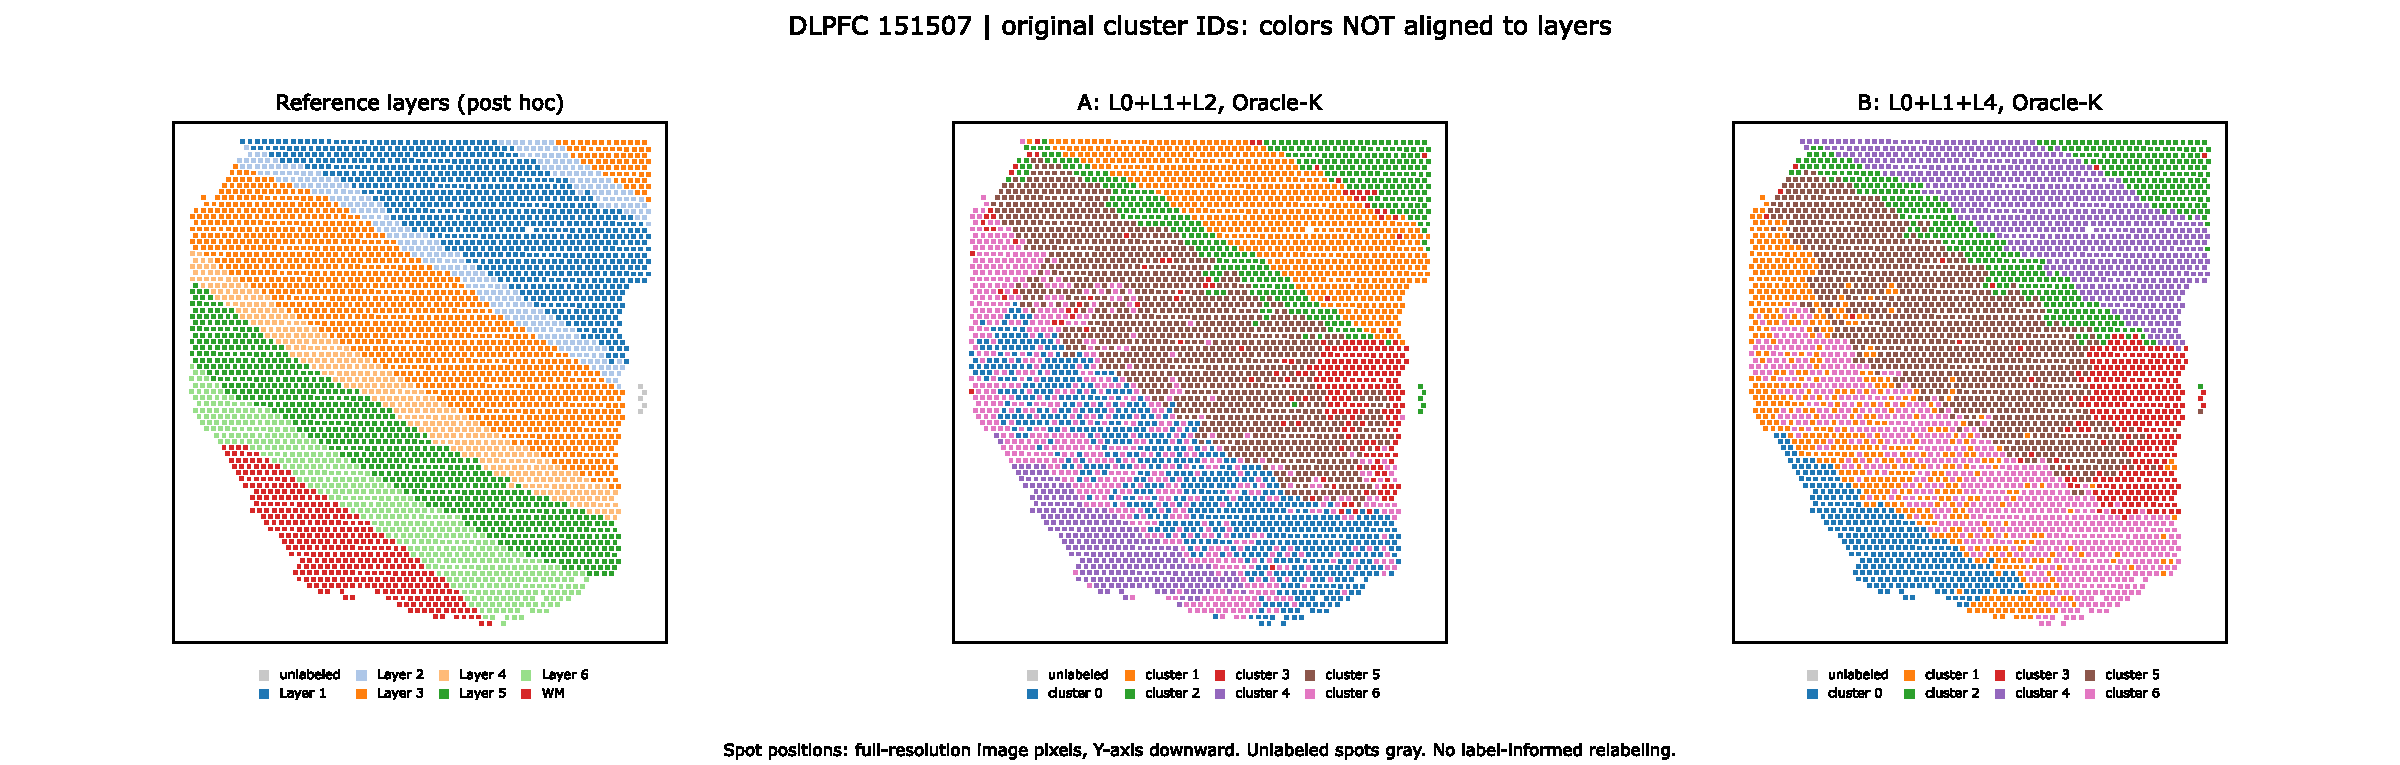
\includegraphics[width=0.98\linewidth]{E4_SOURCE_FIGURES_20261122_RELEASE/figures_pdf/151507/151507_reference_A_B_spatial.pdf}
\caption{DLPFC切片151507的参考层及A、B两种15维组合的聚类结果（第一名供体中B相对A为正向的代表切片；颜色不代表经标签对齐的簇）}
\label{fig:cc-e4-151507-p1}
\end{figure}
}{\par\noindent\emph{[编译提示：未找到151507空间三联图的PDF，请检查相对路径。]}\par}
\IfFileExists{E4_SOURCE_FIGURES_20261122_RELEASE/figures_pdf/151671/151671_reference_A_B_spatial.pdf}{%
\begin{figure}[htbp]
\centering
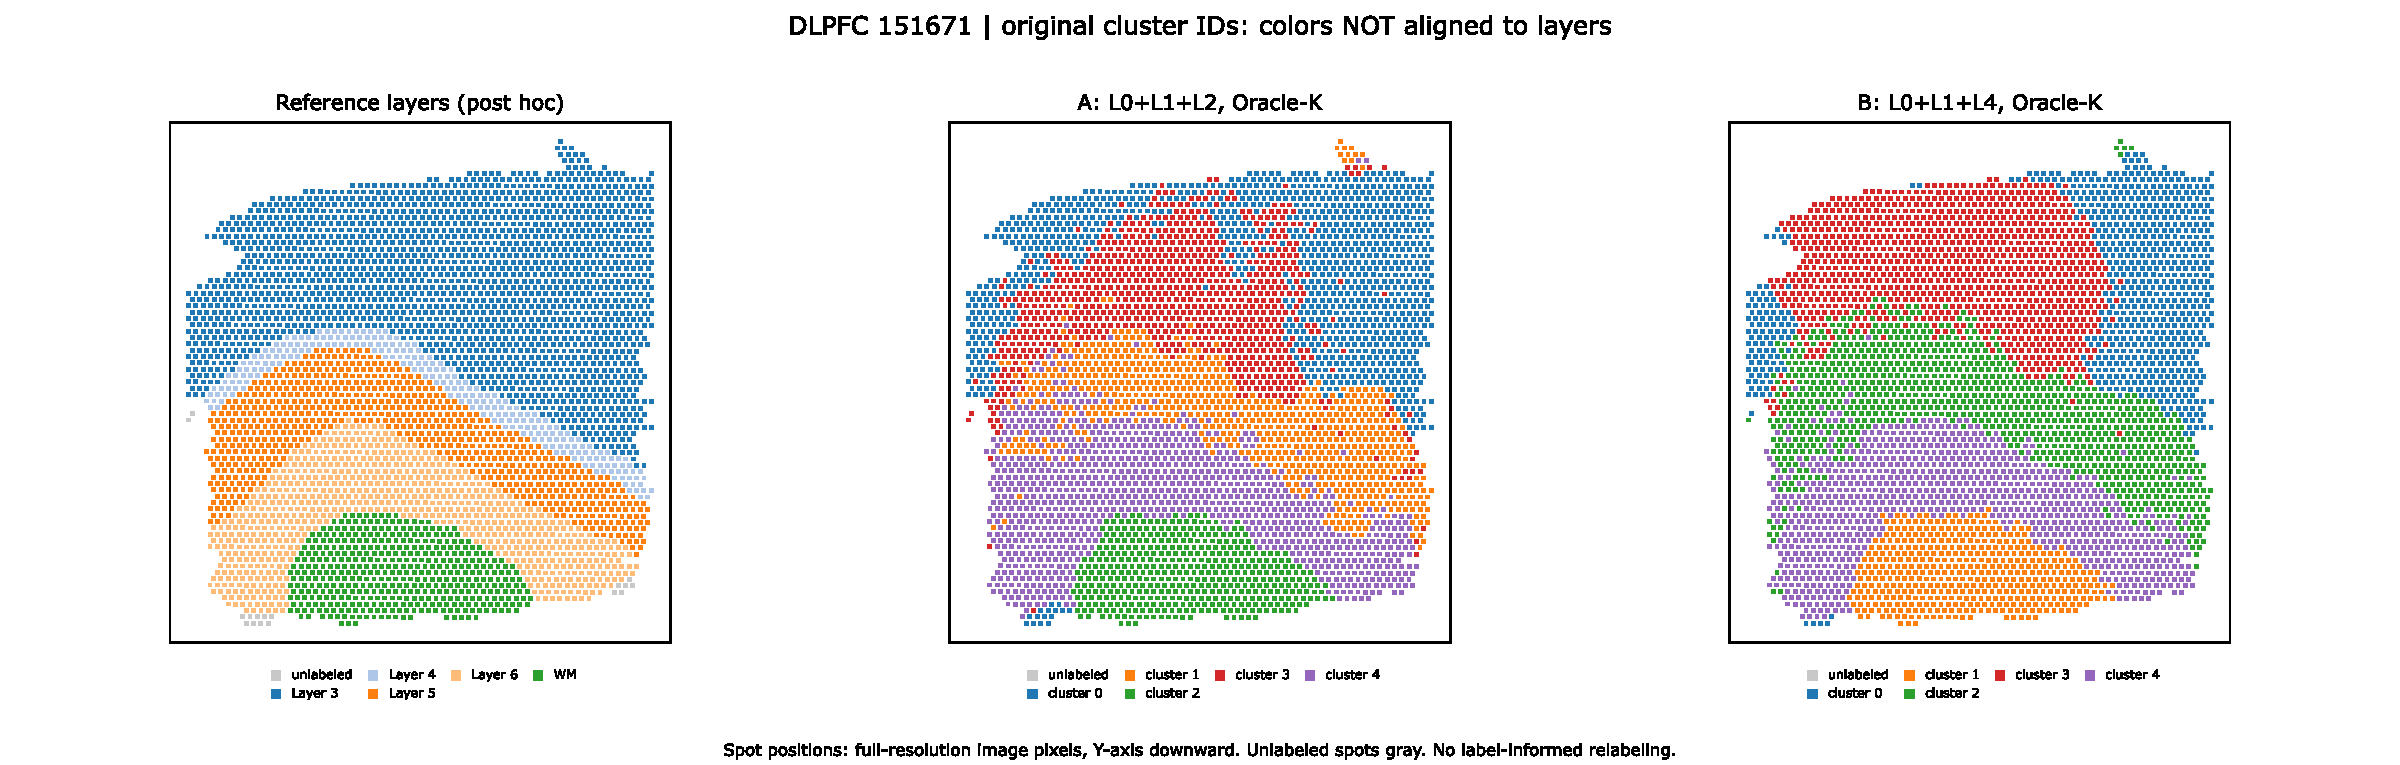
\includegraphics[width=0.98\linewidth]{E4_SOURCE_FIGURES_20261122_RELEASE/figures_pdf/151671/151671_reference_A_B_spatial.pdf}
\caption{DLPFC切片151671的参考层及A、B两种15维组合的聚类结果（第二名供体中B相对A接近零的代表切片）}
\label{fig:cc-e4-151671-p1}
\end{figure}
}{\par\noindent\emph{[编译提示：未找到151671空间三联图的PDF，请检查相对路径。]}\par}
\IfFileExists{E4_SOURCE_FIGURES_20261122_RELEASE/figures_pdf/151675/151675_reference_A_B_spatial.pdf}{%
\begin{figure}[htbp]
\centering
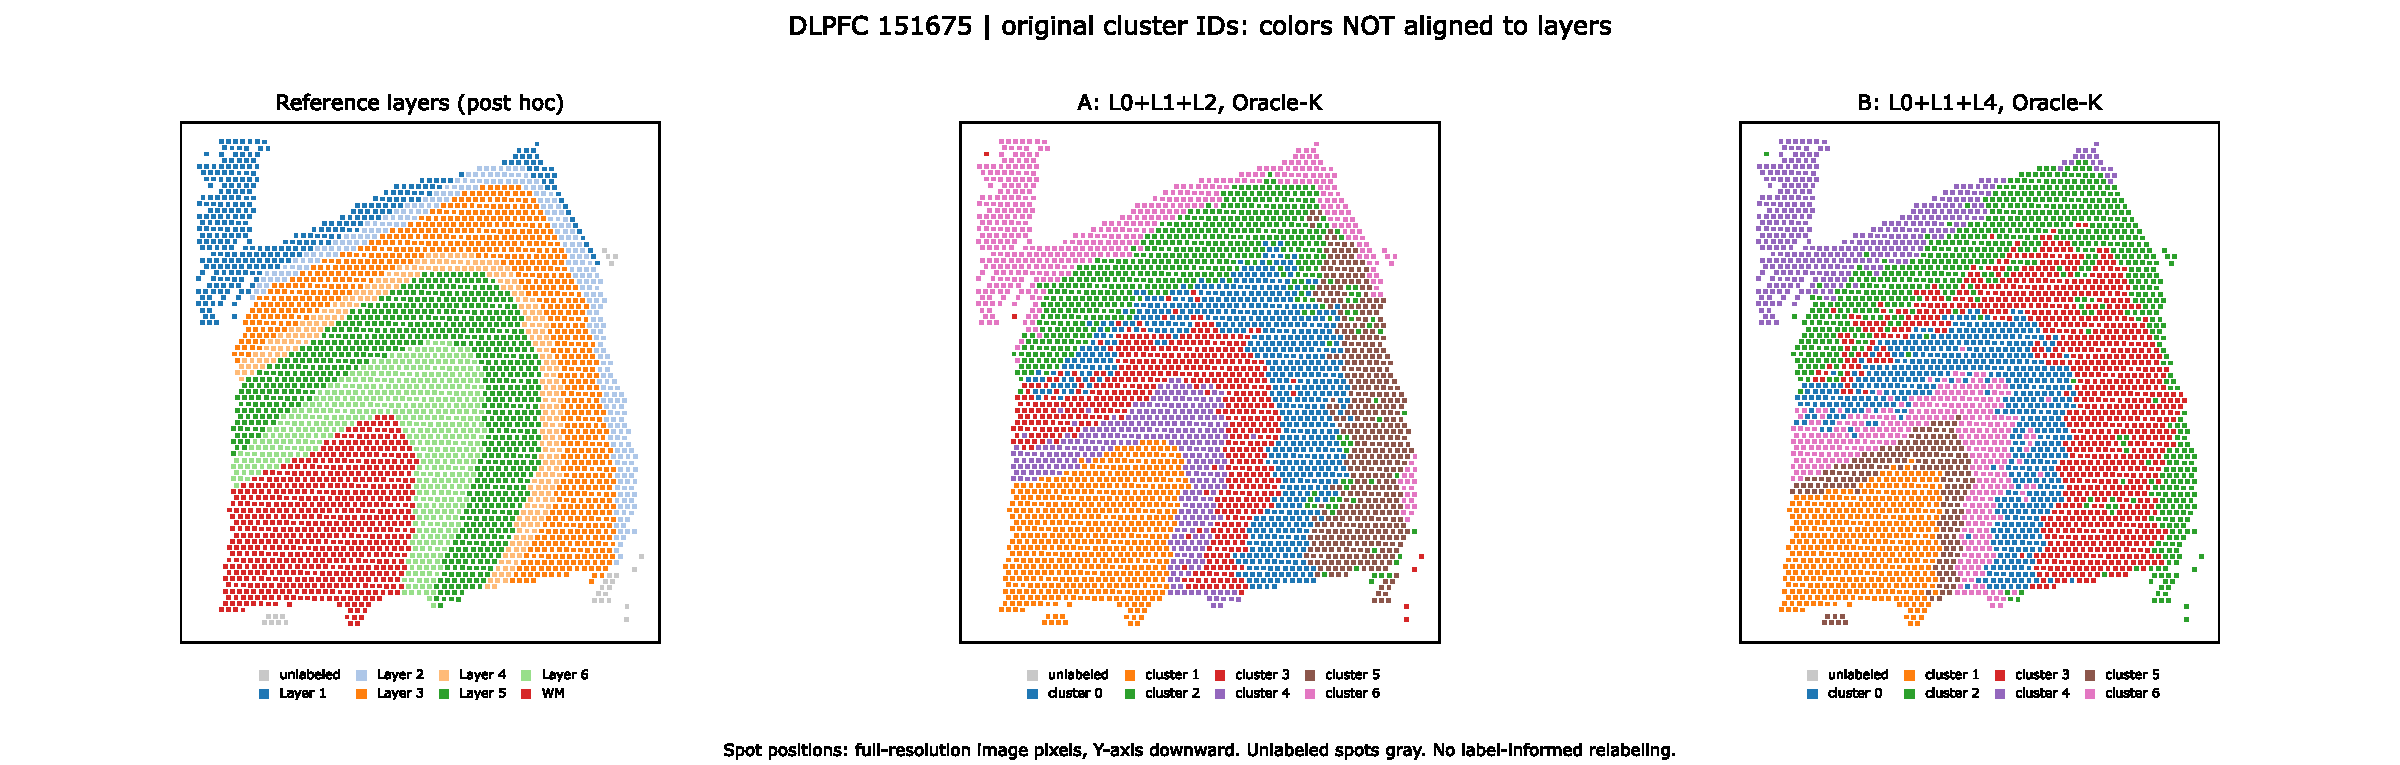
\includegraphics[width=0.98\linewidth]{E4_SOURCE_FIGURES_20261122_RELEASE/figures_pdf/151675/151675_reference_A_B_spatial.pdf}
\caption{DLPFC切片151675的参考层及A、B两种15维组合的聚类结果（第三名供体中B相对A为负向的代表切片）}
\label{fig:cc-e4-151675-p1}
\end{figure}
}{\par\noindent\emph{[编译提示：未找到151675空间三联图的PDF，请检查相对路径。]}\par}
\IfFileExists{E4_SOURCE_FIGURES_20261122_RELEASE/figures_pdf/151671/151671_MOBP_PCP4_SNAP25_expression.pdf}{%
\begin{figure}[htbp]
\centering
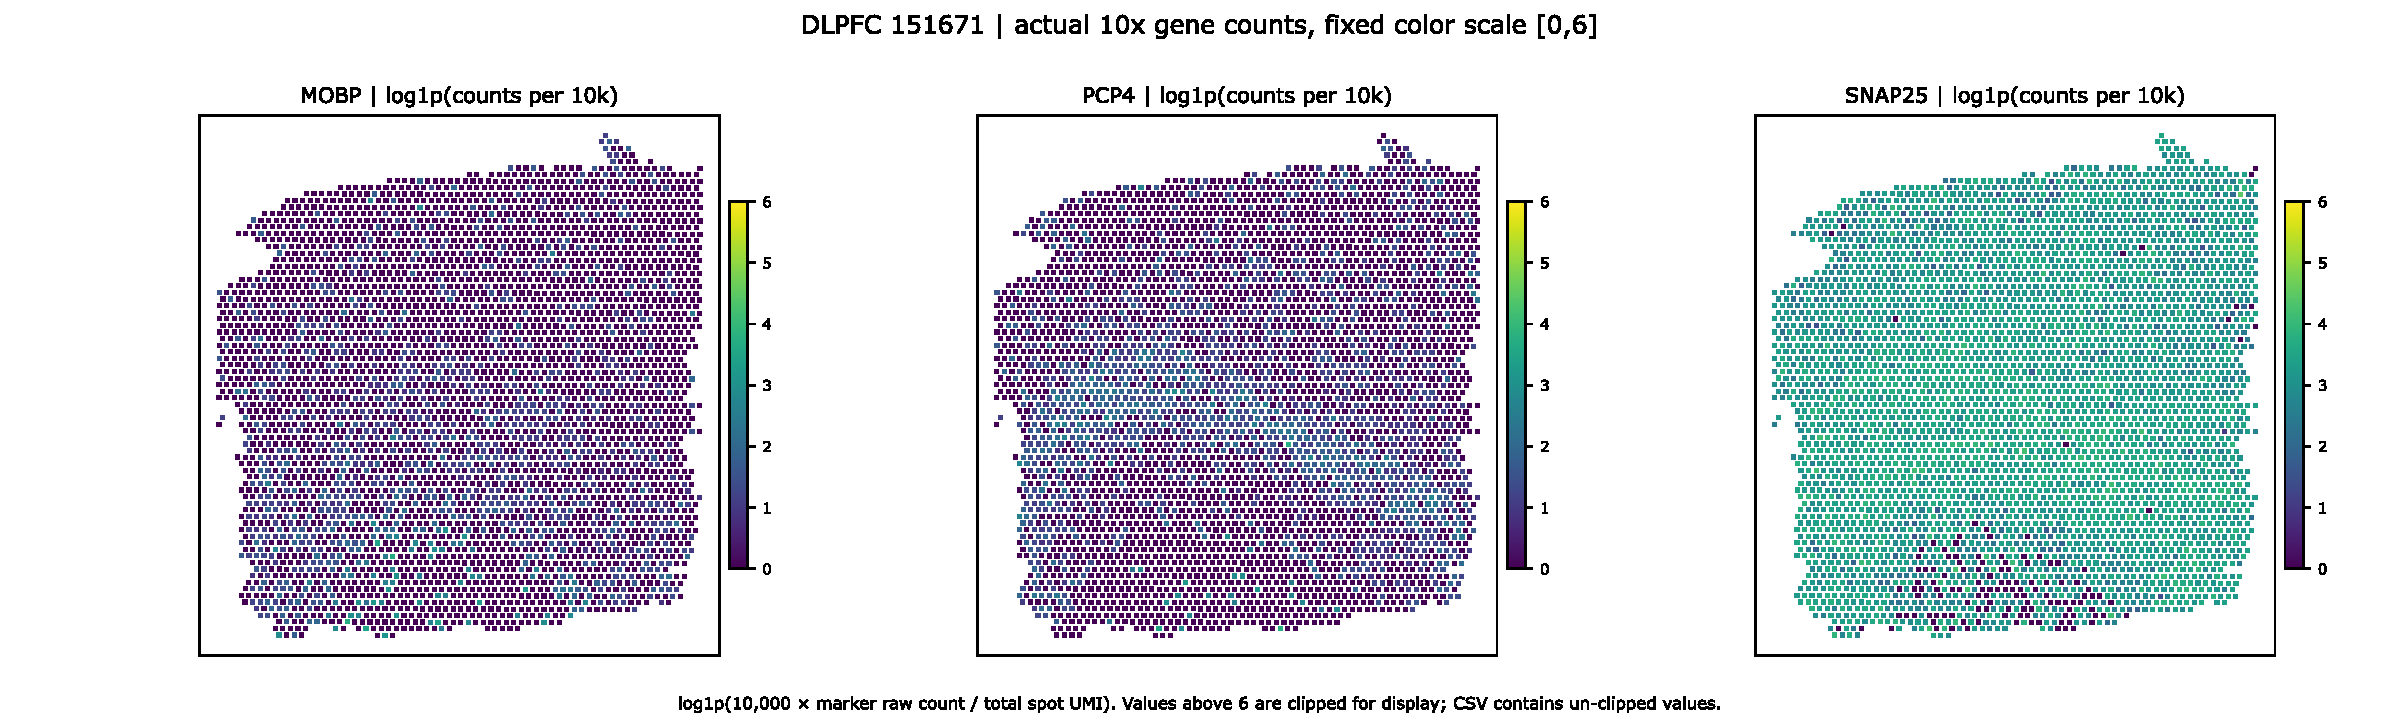
\includegraphics[width=0.98\linewidth]{E4_SOURCE_FIGURES_20261122_RELEASE/figures_pdf/151671/151671_MOBP_PCP4_SNAP25_expression.pdf}
\caption{DLPFC切片151671中MOBP、PCP4与SNAP25的归一化表达空间分布（统一的0--6色标）}
\label{fig:cc-e4-markers-151671-p1}
\end{figure}
}{\par\noindent\emph{[编译提示：未找到151671标记基因图的PDF，请检查相对路径。]}\par}

\subsection{讨论}
\label{subsec:cc-discussion-p1}

\subsubsection{同一方法的结论为何随条件而变}
以上结果显示，“邻域越大越好”这一结论只在特定的组合条件下成立：参考类别数确定K、以整体一致性或容差边界评价、观察宏平均。可以从三个方面理解其原因。
\begin{itemize}
  \item \textbf{邻域信息的边际收益递减。}一种合理的解释是：第一层邻域汇聚了相邻spot的表达，减弱了单spot表达的噪声，因此带来一致的提升；更远的邻域层与已有信息的重叠较多，增益随之变小。对于层厚不同的切片，更远的邻域还可能跨越层界，这与供体D3的反向趋势相容。以上解释都没有经过本研究的直接检验。
  \item \textbf{K的设定与尺度效应相互叠加。}固定K时，尺度排序稳定；一旦K由数据自行决定，选中K的波动（2到10）就压过了尺度之间的细小差别，排序随之改变。参考类别数并非ARI最优的K，这进一步说明，在参考类别数条件下得到的尺度比较，隐含地依赖于“K等于参考类别数”这一约定。
  \item \textbf{整体指标与严格边界指标衡量的是不同的误差。}随着邻域加深，预测边界的数量明显减少，预测分区更加平滑，整体一致性和容差边界匹配随之提高；而在严格网格匹配下，平滑后的边界只要错开一两个位置就不再计为命中，严格召回因此下降。两类指标的相反趋势，是同一组预测在不同评价问题上的表现，而不是互相矛盾的结论。
\end{itemize}

\subsubsection{对方法使用与评价的建议}
在本研究的数据与条件范围内，可以得到以下建议：
\begin{enumerate}
  \item \textbf{邻域层数。}在Visium皮层数据上，1--2层邻域已能获得大部分ARI收益；更深的聚合可以作为候选，但应报告其在切片或供体层面的方向，而不是只报告宏平均。
  \item \textbf{聚类数。}参考类别数条件下的结果应与固定K敏感性曲线一起报告。使用无标签稳定性选K时，宜采用足够的重复次数，并检查选中K是否落在搜索边界上；比较方法时，应同时列出各方法实际采用的选K规则。
  \item \textbf{边界评价。}应同时报告严格与容差边界指标，并给出precision、recall或预测边界数量，以区分定位偏移和预测碎片化。
  \item \textbf{跨数据集应用。}应逐个报告供体或患者的结果；宏平均容易被个别样本主导，在乳腺癌队列中，单个患者就足以改变配置之间的排序。
\end{enumerate}

\subsubsection{与已有研究的关系}
本研究的参考类别数结果与CellCharter原作者的单切片基准处于同一水平，也与原作者在调参中选择4层邻域相一致\cite{varrone2024}。在此基础上，本研究进一步说明：这一选择所带来的平均增益，在第一层之后已经较小，且依赖于聚类数设定和评价指标。原作者报告BIC倾向于给出更多的簇；本研究在非空间GMM基线上观察到同样的现象（32/36项选到上界）。已有的空间聚类评价研究强调，方法排序会因数据处理和参数设定而改变\cite{sun2026}；本研究在同一方法内部的尺度比较上，给出了相应的实证例子。

\subsubsection{研究局限}
\label{subsubsec:cc-limits-p1}
本研究的结论受到以下限制：
\begin{enumerate}
  \item DLPFC只有3名独立供体，乳腺癌只有6名患者，结论以描述性的分层统计为主，不作显著性推断；供体映射依据公开资料推定。
  \item 25维配置由原作者依据参考标签在3张切片上调出，组合B在开发切片上提出，这些切片都不是未接触样本；正文对相应结果分别报告了不同的汇总口径。
  \item 累计邻域深度与特征维数同时变化，等维组合只能部分区分两者的影响；边界分析没有零模型基准，相关解释不涉及因果机制。
  \item 稳定性选K只做了5次重复且逐切片运行；BayesSpace与GMM的K-blind似然规则大量命中搜索上界，其中BayesSpace的规则与官方建议不一致；对照集未包含STAGATE。这些因素限制了K-blind条件下方法比较的结论范围。
  \item 无标签选K的评分、边界指标、排除开发切片的汇总、与官方结果的对照以及K偏好分析，都是事后分析，只用于解释和检验稳健性，不是独立验证。
  \item 皮层层标注与乳腺癌病理区域的语义不同，不比较两种组织之间的ARI绝对值；外部队列的结果也不代表临床诊断性能。
\end{enumerate}

\subsection{本节小结}
本节表明，CellCharter的邻域聚合在DLPFC上带来明确的收益，收益主要集中在第一层邻域；更深的聚合只有小幅且因切片而异的增益。聚类数的设定对结论的影响大于15维之后的尺度差异，参考类别数也并非ARI最优的K。整体一致性与严格边界定位呈现相反的尺度排序，这主要源于预测碎片化程度的变化。在乳腺癌队列中，空间邻域特征相对非空间表示的收益方向得到保留，但患者间差异很大，与BayesSpace的比较随指标和K规则而变。这些结果共同说明，对成熟空间聚类方法的性能判断，应同时考虑聚类数规则、评价指标和样本层级。
